\documentclass[a4paper,10pt]{article}
\usepackage[utf8]{inputenc}
\usepackage{listings}
\usepackage{graphicx}
\usepackage{xcolor}
\lstset{
  basicstyle=\ttfamily,       % the size of the fonts that are used for the code
  numbers=left,                   % where to put the line-numbers
  numberstyle=\footnotesize,      % the size of the fonts that are used for the line-numbers
  stepnumber=1,                   % the step between two line-numbers. If it is 1 each line will be numbered
  numbersep=5pt,                  % how far the line-numbers are from the code
  backgroundcolor=\color{white},  % choose the background color. You must add \usepackage{color}
  showspaces=false,               % show spaces adding particular underscores
  showstringspaces=false,         % underline spaces within strings
  showtabs=false,                 % show tabs within strings adding particular underscores
  %frame=single,                   % adds a frame around the code
  tabsize=2,                      % sets default tabsize to 2 spaces
  captionpos=b,                   % sets the caption-position to bottom
  breaklines=true,                % sets automatic line breaking
  breakatwhitespace=false,        % sets if automatic breaks should only happen at whitespace
  escapeinside={\%*}{*)},         % if you want to add a comment within your code
  commentstyle=\color{red},
  %keywordstyle=\color{blue}
}

\title{Rechnernetze Aufgabe 3 Auswertung}
\author{
  Triebe, Marian\\
  \texttt{marian.triebe@haw-hamburg.de}
  \and
  Kirstein, Katja\\
  \texttt{katja.kirstein@haw-hamburg.de}
}

\begin{document}

\maketitle
\tableofcontents
\newpage

\section{Routingtabellen}
Das erstellen der Routingtabellen verlief wie geplant, jedoch stellte sich die Frage, ob
die Rechner (R1-R7) aus den internen Netzen mit R8 kommunizieren dürfen. Wir nehmen an, dass R8
einen Rechner aus dem Internet darstellen soll, da R8 auch nicht im Topologie-Plan gelistet ist.
Die Rechner aus den internen Netzen erreichen R8 somit über die default Routings ihres jeweiligen Routers.\\
\newline
Kritisch waren die Routingtabellen für R6 sowie R2, da darauf geachtet werden musste, dass das 172.16.12.0/24 Netz
nur über das VPN Netzwerk (172.16.15.0/24) erreichbar sein darf. Somit ist gewehrleistet das die SSH Verbindung von R7
in die DMZ (R3) nicht über das Internet geroutet wird.\\
\newline
Das korrekte Routing über die einzelnen Knoten wurde mit \textit{tracert} sowie \textit{ping} geprüft.

\section{Portscan DMZ (ohne Firewall)}
Der Portscan ergab, dass auf R3 die folgenden Dienste aktiv sind:
\begin{itemize}
 \item FTP (21)
 \item SSH (22)
 \item HTTP (80)
\end{itemize}
Dies entspricht dem erwarteten Verhalten, da R3 einen SSH-daemon, FTP sowie HTTP bereitstellt. Der Portscan wurde
durch den Befehl \textit{nmap -P0 -p1-99 r3\_0} angestartet und hat die Port-range 1 bis 99 gescannt. Gestartet wurde
\textit{nmap} von R1.

\section{Einstellen der Policy}
Die default Policy der Ketten \textit{INPUT, OUTPUT, FORWARD} wurden auf \textit{DROP} gestellt (Listing 1).
\begin{lstlisting}[language=bash,caption={Default Policy}]
## Default Policy DROP
iptables -P INPUT   DROP
iptables -P OUTPUT  DROP
iptables -P FORWARD DROP
\end{lstlisting}
Dies hatte zur folge, dass \textit{nmap} keine freien Ports mehr scannen konnte, außerdem war es nicht mehr möglich
einen anderen Rechner per \textit{ping} zu erreichen. Generell wurden alle Pakete automatisch verworfen, da es keine
Ausnahmeregeln gab.

\section{Ping erlauben}
Teil der Aufgabe ist es, innerhalb der internen Netzwerke sowie von internen Netzwerken in das Internet zu pingen. Es sollen
jedoch keine Pings aus dem Internet an PCs in internen Netzwerken weitergeleitet werden.\\
Es ist somit notwenig bei jedem PC in den internen Netzwerken eingehende ICMP Pakete zu erlauben (Listing 2).
\begin{lstlisting}[language=bash,caption={ICMP eingehend/ausgehend}]
## Ping senden
iptables -A INPUT   -p icmp --icmp-type echo-request -j ACCEPT
iptables -A OUTPUT  -p icmp --icmp-type echo-request -j ACCEPT
## Ping antwort
iptables -A INPUT   -p icmp --icmp-type echo-reply -j ACCEPT
iptables -A OUTPUT  -p icmp --icmp-type echo-reply -j ACCEPT
\end{lstlisting}
Die Rechner R2, R4 sowie R6 benötigten zusätzlich die Erlaubnis Pakete die nur weitergeleitet werden sollen zu akzeptieren (Listing 3).
\begin{lstlisting}[language=bash,caption={ICMP Weiterleitung}]
## Ping senden
iptables -A FORWARD -p icmp --icmp-type echo-request -j ACCEPT
## Ping antwort
iptables -A FORWARD -p icmp --icmp-type echo-reply -j ACCEPT
\end{lstlisting}
Das filtern von ICMP Paketen von fremden Netzwerken (bspw. aus dem Internet) geschieht bei R5. Hierzu haben wir die \textit{-i} Option
von \textit{iptables} verwendet. Diese Option bezieht das Interface auf welchem das Paket empfangen wurde mit ein (Listing 4). Zum
filtern fremder Pakete wurde es einfach nicht erlaubt Pakete vom Typ \textit{echo-request} von Interface \textit{eth2} freizugeben,
das hat zur folge, dass die Pakete korrekt gefiltert werden.
\begin{lstlisting}[language=bash,caption={ICMP filter}]
## Filter fuer Internes Netz / Internet Pings
iptables -A FORWARD -i eth0 -p icmp --icmp-type echo-reply -j ACCEPT
iptables -A FORWARD -i eth0 -p icmp --icmp-type echo-request -j ACCEPT
iptables -A FORWARD -i eth1 -p icmp --icmp-type echo-reply -j ACCEPT
iptables -A FORWARD -i eth1 -p icmp --icmp-type echo-request -j ACCEPT
iptables -A FORWARD -i eth2 -p icmp --icmp-type echo-reply -j ACCEPT
\end{lstlisting}

\newpage

\section{SSH in die DMZ}
Es ist nur von R1 sowie R7 möglich eine SSH Verbindung in die DMZ (zu R3) aufzubauen. Dazu musste R3 so konfiguriert werden, dass
eingehende SSH Verbindungen akzeptiert werden (Listing 5). Es werden nur Verbindungen von R1 und R7 zugelassen, das wird durch die
\textit{-s ip} Option von \textit{iptables} sichergestellt.
\begin{lstlisting}[language=bash,caption={SSH eingehend/ausgehend}]
## R1
iptables -A INPUT  -p tcp -s 172.16.11.1 --sport 513:65535 --dport 22 -m state --state NEW,ESTABLISHED -j ACCEPT
## R7
iptables -A INPUT -p tcp -s 172.16.14.2 --sport 513:65535 --dport 22 -m state --state NEW,ESTABLISHED -j ACCEPT
\end{lstlisting}
Desweiteren musste die Weiterleitung von SSH Paketen erlaubt werden. Dies musste auf R2 sowie R6 konfiguriert werden (Listing 6).
Die Konfiguration von R6 ist Identisch mit der von R2, jedoch kann die Regel zum weiterleiten der Pakete von R1 nach R3 entfallen,
da Pakete von R1 nicht über R6 geroutet werden.
\begin{lstlisting}[language=bash,caption={SSH Weiterleitung (Konfiguration von R2)}]
## R1
iptables -A FORWARD -p tcp -s 172.16.11.1 -d 172.16.12.2 --sport 513:65535 --dport 22 -m state --state NEW,ESTABLISHED -j ACCEPT
iptables -A FORWARD -p tcp -s 172.16.12.2 -d 172.16.11.1 --sport 22 --dport 513:65535 -m state --state ESTABLISHED -j ACCEPT
## R7
iptables -A FORWARD -p tcp -s 172.16.14.2 -d 172.16.12.2 --sport 513:65535 --dport 22 -m state --state NEW,ESTABLISHED -j ACCEPT
iptables -A FORWARD -p tcp -s 172.16.12.2 -d 172.16.14.2 --sport 22 --dport 513:65535 -m state --state ESTABLISHED -j ACCEPT
\end{lstlisting}
Die Verbindung von R1 zu R3 erfolg ausschließlich über die internen Netzwerke, wie in Figure 1 zu sehen.
Selbiges gilt für Verbindungen von R7 zu R3, in Figure 2 zu sehen.
\begin{figure}[h]
  \centering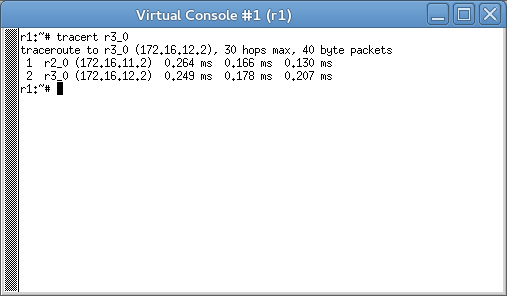
\includegraphics[scale=.5]{tracert_r1_to_r3.png}
  \caption{tracert zu R3 von R1}
\end{figure}
\begin{figure}[h]
  \centering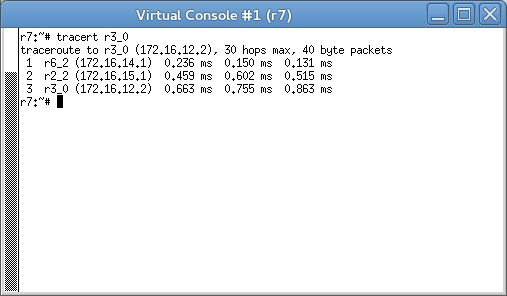
\includegraphics[scale=.5]{tracert_r7_to_r3.png}
  \caption{tracert zu R3 von R7}
\end{figure}

\newpage

\section{Stateful Firewall}
Mit Hilfe der Stateful Option von \textit{iptables} ist es möglich Verbindungen die in bestimmten Zuständen sind zu erlauben. Bspw. wenn
bei einem TCP Paket das SYN Flag gesetzt ist, oder eine Verbindung bereits aufgebaut wurde (ESTABLISHED). Wir erlauben alle Pakete die
bereits zu einer bestehenden Verbindung zugeordnet werden können (Listung 7).
\begin{lstlisting}[language=bash,caption={Stateful ESTABLISHED,RELATED}]
iptables -A INPUT   -m state --state ESTABLISHED,RELATED -j ACCEPT
iptables -A OUTPUT  -m state --state ESTABLISHED,RELATED -j ACCEPT
iptables -A FORWARD -m state --state ESTABLISHED,RELATED -j ACCEPT
\end{lstlisting}
Außerdem erlauben wir TCP Verbindungen zu Port 20, 21 sowie 80 bei denen das SYN Flag gesetzt wurde. Dies in Verbindung mit den Regeln
aus Listing 6 erlaubt HTTP, sowie FTP Verbindungen.
\begin{lstlisting}[language=bash,caption={Stateful NEW, SYN FLAG}]
iptables -A FORWARD -m state --state NEW -p tcp --syn --dport 20 -j ACCEPT
iptables -A FORWARD -m state --state NEW -p tcp --syn --dport 21 -j ACCEPT
iptables -A FORWARD -m state --state NEW -p tcp --syn --dport 80 -j ACCEPT
\end{lstlisting}
Desweiteren mussten auf R3 eingehende Pakete für Port 20, 21 sowie 80 akzeptiert werden. Hierzu haben wir die Regeln aus Listing 7 leicht angepasst.
Zum anpassen der Regel wurde das \textit{FORWARD} Keyword durch \textit{INPUT} ersetzt.\\
\newline
Die HTTP Verbindung zu R3 von externen Netzwerken (R8) ist erfolgreich und wurde mit der Hilfe des Programms \textit{links} getestet (Figure 3).
\begin{figure}[h]
  \centering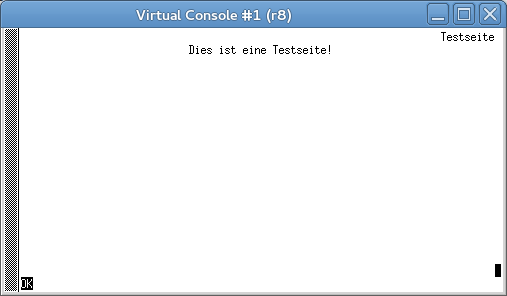
\includegraphics[scale=.5]{http_r8_to_r3.png}
  \caption{HTTP zu R3 von R7 (links http://r3\_0)}
\end{figure}
\begin{figure}[h]
  \centering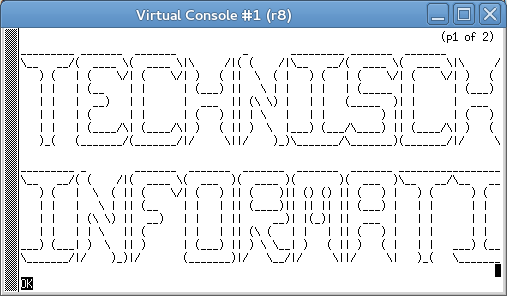
\includegraphics[scale=.5]{ftp_r8_to_r3.png}
  \caption{FTP zu R3 von R7 (links ftp://r3\_0/demo.txt)}
\end{figure}
Die FTP Verbindung zu R3 von externen Netzwerken (R8) ist ebenfalls erfolgreich und wurde mit der Hilfe des Programms \textit{links} getestes (Figure 4).
Von internen Hosts (r1 bis r7) war ebenfalls der Zugriff auf die HTTP, FTP Dienste von R3 möglich.

\end{document}